% Standalone living guide: no external figures or input files required.
% Update the revision/date and revision record whenever capabilities change.
\documentclass[11pt,a4paper]{article}
\usepackage[T1]{fontenc}
\usepackage[margin=25mm]{geometry}
\usepackage{amsmath,amssymb,booktabs,longtable,array}
\usepackage{xcolor,listings}
\usepackage{tikz}
\usetikzlibrary{arrows.meta,positioning,decorations.markings}
\usepackage{hyperref}
\hypersetup{colorlinks=true,linkcolor=blue!45!black,urlcolor=blue!45!black}
\newcommand{\GuideVersion}{0.7}
\newcommand{\GuideDate}{8 October 2026}
\newcommand{\He}{\ensuremath{{}^{3}\mathrm{He}}}
\let\file\path
\lstset{basicstyle=\ttfamily\small,breaklines=true,columns=fullflexible,
 keepspaces=true,frame=single,rulecolor=\color{black!20},
 backgroundcolor=\color{black!2},showstringspaces=false}
\setlength{\parindent}{0pt}
\setlength{\parskip}{6pt}
\setlength{\emergencystretch}{3em}
\title{FermiForge\\\large A hands-on map of the framework}
\author{Living project documentation}
\date{Revision \GuideVersion\ --- \GuideDate}
\begin{document}
\maketitle
\begin{abstract}
This guide connects the physical calculation, software layers and day-to-day
workflow of FermiForge. It distinguishes general two-dimensional free-vortex
calculations from symmetry-constrained radial and cylinder modes, maps the
source modules, and gives small practical exercises. It describes the
implementation at the revision date, not a promise that every parameter
regime or planned device geometry has been validated.
\end{abstract}
\tableofcontents
\clearpage

\section{Scope and present capabilities}
The present solver is a spinful quasiclassical mean-field solver for \He.
Fields depend on $x,y$ and are translation-invariant along $z$, but momentum
retains three components. Spatially two-dimensional therefore does not mean
a two-dimensional Fermi surface.

The modern transport and self-consistency solver is Fortran. Python prepares,
archives, diagnoses and plots runs. The separate \file{new_src} radial code is
a numerical reference, not the engine underneath every modern run.
At each independent point the state contains nine complex components
$A_{\mu i}$ (spin index $\mu$, orbital index $i$) and three real current-related
Fermi-liquid fields: 21 real iteration entries. Propagation retains spin
structure. The current self-consistency law is the \He\ model; a general
library of superconducting materials and interfaces remains a development goal.

\begin{center}\small
\begin{tabular}{p{.23\linewidth}p{.32\linewidth}p{.34\linewidth}}
\toprule Calculation & Route & Constraint \\\midrule
General 2D free vortex & Axisymmetric benchmark in \file{full_2d}, or double-core driver & No cylindrical field symmetry \\
Radial free vortex & \file{radial_symmetry} mode & Independent positive-$x$ ray; angular reconstruction imposed \\
Specular cylinder & Modern cylinder driver & Radial or experimental unrestricted uniform-grid disk; reflected trajectories \\
Legacy reference & \file{new_src} & Separate radial solver and conventions \\
Manufactured demo & 2D demo & Prescribed fields; no self-consistency \\\bottomrule
\end{tabular}\end{center}

The name \file{benchmark_axisymmetric_core_2d} is historical: in
\file{full_2d} mode it evolves an unconstrained planar field even when the
initial state is axisymmetric. Conversely, plotting a radial solution over
the plane does not make its calculation unconstrained 2D.

\section{Algorithm and parallel execution}
Figure~\ref{fig:flow} gives the functional sequence. Individual drivers differ:
zero-mode projection and external probes belong to particular free-vortex
workflows, while the cylinder has its own shorter iteration driver.

MPI assigns whole target-point calculations to ranks. A rank handles that
point's momentum directions and energy poles locally. Fields are replicated;
this is not spatial domain decomposition with nearest-neighbour ghost exchange.
The accelerator update is coordinated and the resulting state communicated.
Memory, communication and unequal point costs can eventually limit scaling.

\begin{figure}[p]
\centering
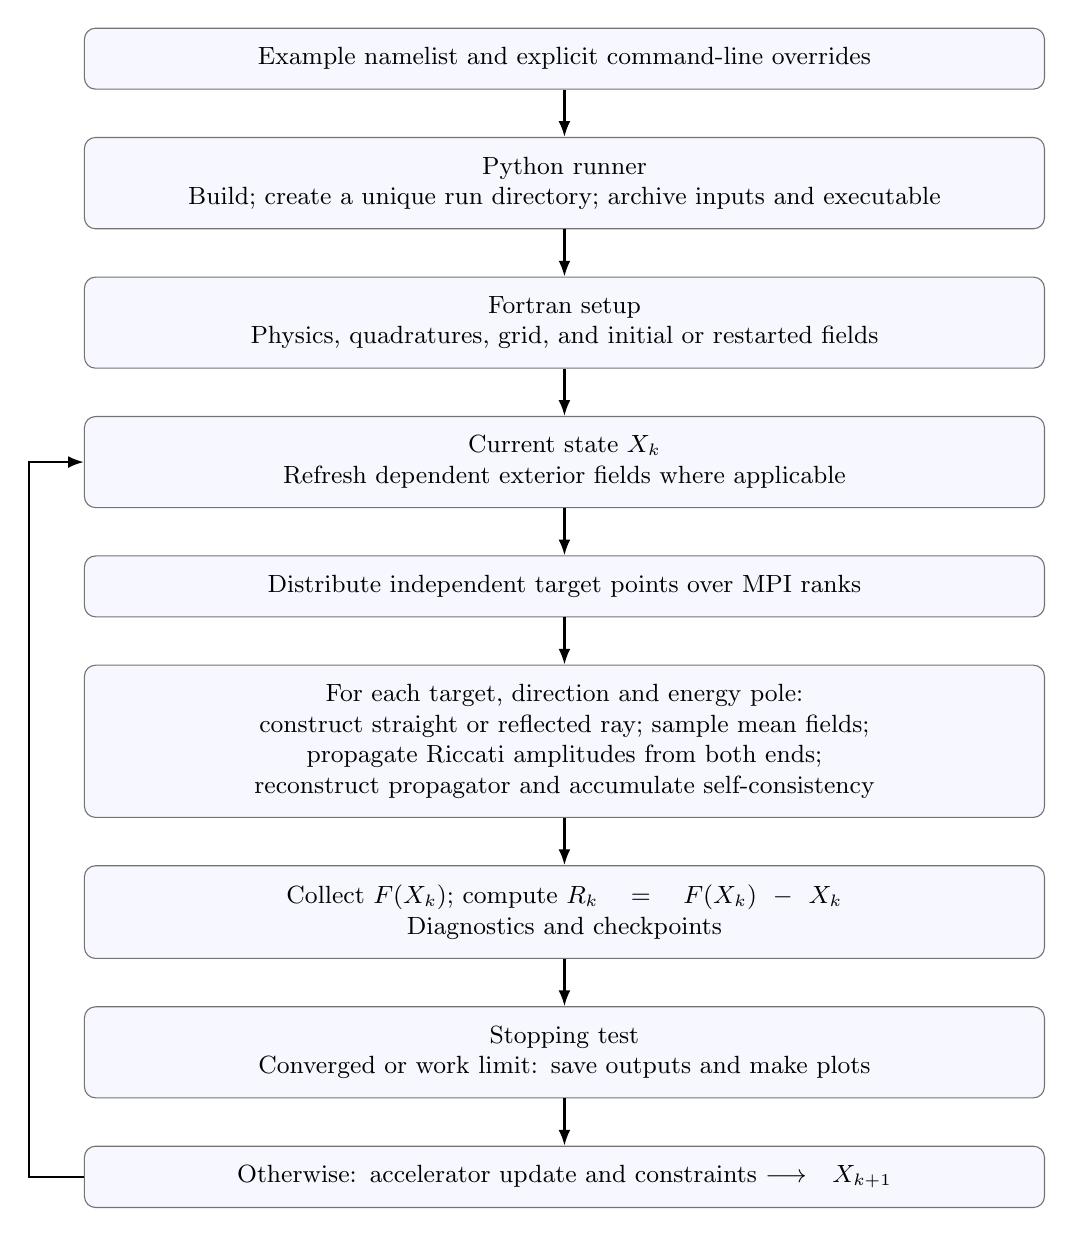
\begin{tikzpicture}[
 node distance=6mm,
 box/.style={draw=black!55,rounded corners,fill=blue!3,text width=11.7cm,
 align=center,inner sep=7pt,font=\small},
 arr/.style={-{Latex[length=2mm]},thick}]
\node[box] (input) {Example namelist and explicit command-line overrides};
\node[box,below=of input] (python) {Python runner\\Build; create a unique run directory; archive inputs and executable};
\node[box,below=of python] (setup) {Fortran setup\\Physics, quadratures, grid, and initial or restarted fields};
\node[box,below=of setup] (state) {Current state $X_k$\\Refresh dependent exterior fields where applicable};
\node[box,below=of state] (mpi) {Distribute independent target points over MPI ranks};
\node[box,below=of mpi] (map) {For each target, direction and energy pole:\\
construct straight or reflected ray; sample mean fields;\\
propagate Riccati amplitudes from both ends;\\
reconstruct propagator and accumulate self-consistency};
\node[box,below=of map] (res) {Collect $F(X_k)$; compute $R_k=F(X_k)-X_k$\\Diagnostics and checkpoints};
\node[box,below=of res] (decision) {Stopping test\\Converged or work limit: save outputs and make plots};
\node[box,below=of decision] (update) {Otherwise: accelerator update and constraints $\longrightarrow X_{k+1}$};
\foreach \a/\b in {input/python,python/setup,setup/state,state/mpi,mpi/map,map/res,res/decision,decision/update}
 \draw[arr] (\a)--(\b);
\draw[arr] (update.west)--++(-.7,0)|-(state.west);
\end{tikzpicture}
\caption{Functional framework map. The loop returns to the current-state stage.
The diagram summarizes the numerical workflow rather than an exact call graph.}
\label{fig:flow}
\end{figure}
\clearpage

\section{Source-code map}
All paths are relative to the repository root. Read a driver first, then follow
the particular layer you want to understand. Long filenames in the table may
wrap; the repository spelling is unchanged.
\begingroup\small
\renewcommand{\arraystretch}{1.2}
\begin{longtable}{p{.30\linewidth}p{.62\linewidth}}
\toprule Layer & Source entry points \\\midrule\endfirsthead
\toprule Layer & Source entry points (continued) \\\midrule\endhead
Run preparation & \path{tools/run_axisymmetric_core_benchmark.py} \\
Free-vortex orchestration & \path{app/benchmark_axisymmetric_core_2d.f90} \\
Double-core orchestration & \path{app/benchmark_legacy_double_core_map_2d.f90}; \path{tools/run_double_core_from_scratch.py} \\
Cylinder & \path{app/benchmark_radial_cylinder_2d.f90}; \path{tools/run_modern_cylinder.py} \\
Mesh and indexing & \path{src/cartesian_mesh_2d.f90} \\
State and radial reconstruction & \path{src/spinful_state_2d.f90} \\
Cartesian sampling & \path{src/bilinear_field_sampler_2d.f90} (historical name) \\
Basis and harmonics & \path{src/order_parameter_basis.f90} \\
Core seeds & \path{src/historical_core_seed_2d.f90} \\
MPI and serial map & \path{src/he3_mpi_field_map_2d.f90}; \path{src/he3_serial_point_map.f90} \\
Straight and reflected rays & \path{src/straight_trajectory_2d.f90}; \path{src/specular_cylinder_2d.f90} \\
Free-vortex exterior & \path{src/free_vortex_asymptotic_2d.f90} \\
Riccati transport & \path{src/legacy_riccati_trajectory_2d.f90}; \path{src/riccati_segment.f90} \\
Propagator and spin algebra & \path{src/quasiclassical_propagator.f90}; \path{src/spin_matrix_2x2.f90} \\
Self-consistency integrand & \path{src/he3_self_consistency_integrand.f90} \\
Quadratures and bulk gap & \path{src/he3_quadrature.f90}; \path{src/ozaki_generator.f90}; \path{src/he3_bulk_gap.f90} \\
Packing and residuals & \path{src/new_src_iteration_layout_2d.f90}; \path{src/he3_nonlinear_iteration_2d.f90} \\
Accelerators & \path{src/legacy_anderson_mixing.f90}; \path{src/barzilai_borwein_mixing.f90}; \path{src/polyak_mixing.f90} \\
Regression coverage & \path{tests/}; registrations in \path{CMakeLists.txt} \\\bottomrule
\end{longtable}\endgroup

\file{examples/} contains inputs; \file{work/} contains builds and working
products; \file{runs/} contains dated experiments; \file{benchmarks/} holds
reference cases. Separately maintained \file{2D_benchmarks/} data may be
absent from another checkout. Do not assume they were uploaded to GitHub.

\section{Grid, trajectories and exterior fields}
\subsection{Independent and dependent points}
The full-2D field grid is tensor-product Cartesian. Uniform, piecewise
multiscale and smoothly stretched choices exist in the appropriate drivers.
The smooth option uses a hyperbolic-sine coordinate mapping, not an
unstructured finite-element mesh or elliptical rings. Active masks and
asymptotic fit surfaces need not coincide with the outer box.

An \emph{active point} receives a self-consistency map and contributes to the
iteration vector. A \emph{dependent halo point} supplies fields for sampling
but may be filled from evolving asymptotics rather than independently relaxed.
External probes test extrapolation; their role and whether they are iterated
depend on the driver and input. They must not silently count as interior
convergence points.

\subsection{Free vortex versus physical wall}
For a free vortex, the phase-wound bulk matrix $A_0$ is the asymptotic
reference. Current-state fitting allows angle-dependent coefficients,
including rotation-like order-parameter tails and inverse-radius mean-field
terms. Reference-based endpoints also exist as comparison tools; they are
not equivalent to \file{state_asymptotic}. The detailed implemented expressions
belong in the mathematical note; this guide does not replace those equations.

Trajectory sampling has its own step size, independent of field-node spacing.
Fewer field points do not imply shorter trajectories. In radial mode,
trajectory fields are interpolated directly from the ray, not the reconstructed
Cartesian plotting grid.

In a cylinder the wall is physical. Rays reflect specularly, remain inside
the wall and use no free-vortex exterior fit. Reflected half-path length is
propagation distance, not cylinder radius. Uniform collision sampling and
collision-aligned sampling are available; finite-step answers need not coincide.

Figure~\ref{fig:cylinder-ray} illustrates one incoming trajectory ending at
an arbitrary off-centre target $\mathbf r_\star$. At a wall point with outward
unit normal $\hat{\mathbf n}$, specular reflection obeys
\begin{equation}
 \hat{\mathbf p}_{\rm out}=\hat{\mathbf p}_{\rm in}
 -2(\hat{\mathbf p}_{\rm in}\cdot\hat{\mathbf n})\hat{\mathbf n},
 \qquad \hat{\mathbf n}=(x/R,y/R,0).
 \label{eq:cylinder-reflection}
\end{equation}
Thus the wall-normal momentum reverses, while tangential momentum and $p_z$
are unchanged. The drawing shows the projection onto the cross-section;
translation invariance of the fields does not restrict the momentum to this
plane. The illustrated starting point is an interior propagation cutoff, not
a reservoir or another boundary condition on the order parameter.

\begin{figure}[htbp]
\centering
% Unit-radius coordinates generated by successive line/circle intersections
% and specular reflection, traced backwards from target (0.52,0.23).
% Incoming target direction: (-0.3,sqrt(0.91)); three reflections.
% Display order is reversed to show propagation towards the target.
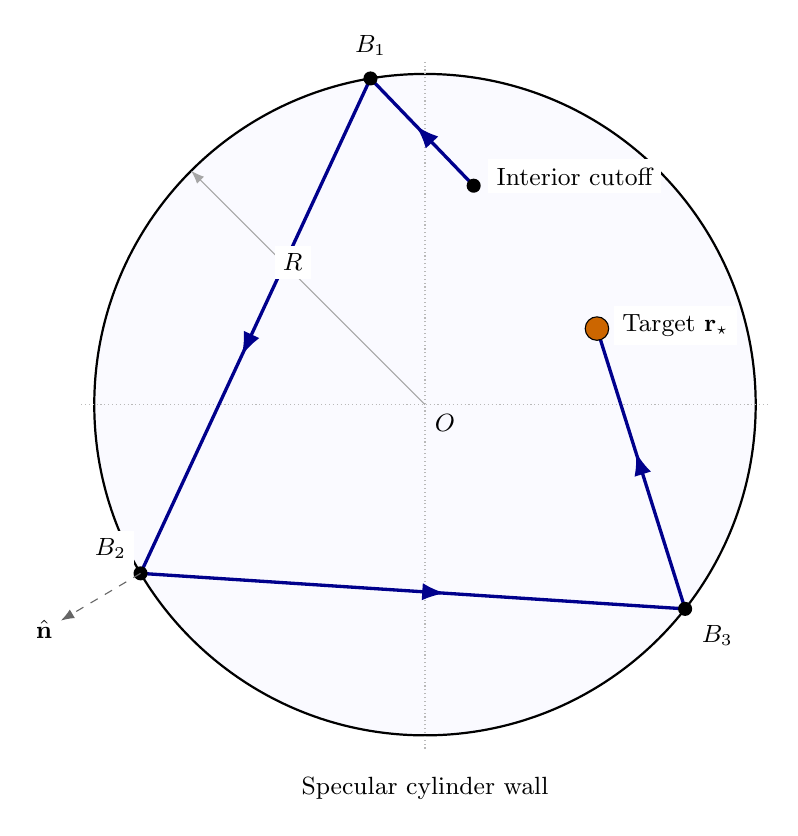
\begin{tikzpicture}[x=4.2cm,y=4.2cm,
 ray/.style={draw=blue!55!black,line width=1.2pt,
 postaction={decorate},decoration={markings,
 mark=at position .56 with {\arrow{Latex}}}},
 dot/.style={circle,fill=black,inner sep=1.8pt},
 lab/.style={font=\small,fill=white,inner sep=3pt}]
\fill[blue!2] (0,0) circle (1);
\draw[thick] (0,0) circle (1);
\draw[gray!55,densely dotted] (-1.04,0)--(1.04,0);
\draw[gray!55,densely dotted] (0,-1.04)--(0,1.04);
\node[font=\small,below right] at (0,0) {$O$};
\coordinate (S) at (0.14717859,0.66203208);
\coordinate (B1) at (-0.16480419,0.98632630);
\coordinate (B2) at (-0.86007890,-0.51016104);
\coordinate (B3) at (0.78653914,-0.61754043);
\coordinate (T) at (0.52000000,0.23000000);
\draw[ray] (S)--(B1);
\draw[ray] (B1)--(B2);
\draw[ray] (B2)--(B3);
\draw[ray] (B3)--(T);
\node[dot] at (S) {};
\node[lab,anchor=west] at (0.19,0.69) {Interior cutoff};
\foreach \p in {B1,B2,B3} \node[dot] at (\p) {};
\node[lab,above=5pt] at (B1) {$B_1$};
\node[lab,below right=4pt] at (B3) {$B_3$};
\node[lab,above left=3pt] at (B2) {$B_2$};
\draw[black!60,dashed,-{Latex}] (B2)--(-1.101,-0.653);
\node[lab,anchor=east] at (-1.10,-0.68) {$\hat{\mathbf n}$};
\node[circle,fill=orange!80!black,draw=black,inner sep=3pt] at (T) {};
\node[lab,anchor=west] at (0.57,0.24) {Target $\mathbf r_\star$};
\draw[gray!70,-{Latex}] (0,0)--(-0.70710678,0.70710678);
\node[lab] at (-0.40,0.43) {$R$};
\node[lab,anchor=north] at (0,-1.10) {Specular cylinder wall};
\end{tikzpicture}
\caption{One incoming trajectory in the circular cross-section, shown with
three exact specular reflections $B_1\to B_2\to B_3$ before reaching the
off-centre target. Arrows indicate propagation towards the target; the dashed
arrow is the outward wall normal at $B_2$. Coordinates are normalized by $R$.
The full propagator calculation uses both trajectory halves, propagated from
their respective remote ends to the target; only one half is drawn for clarity.
This geometry is shared by the radial field sampler and the experimental
interior-only disk sampler (Cartesian or annular nodes).}
\label{fig:cylinder-ray}
\end{figure}

\section{Input controls}
\subsection*{A-phase texture trial states}
For full 2D cylinders, \file{--initialization -2 --texture a_mermin_ho}
sets $\mathbf d=\mathbf e_z$ and
\[
 A_{\mu i}=C d_\mu e^{i\phi}
 [\cos\beta\,e_{r,i}-\sin\beta\,e_{z,i}+i e_{\phi,i}],\qquad
 \beta=\frac{\pi r}{2R}.
\]
The centre is evaluated explicitly as $A_{zi}=C(1,i,0)$; all other rows
vanish initially. This smooth pure-A seed has
$\boldsymbol\ell=\sin\beta\,\mathbf e_r+\cos\beta\,\mathbf e_z$ and
$v_{s,\phi}=\hbar(1-\cos\beta)/(2m_3r)$: one circulation quantum at
the wall, without a singular core. The legacy input \file{winding=0}
means no additional imposed phase factor here, not zero total circulation.
The initial scale $C=\sqrt2\Delta_B^{\rm legacy}(T)$ matches the old uniform
A seed; it is not a separately solved A-phase bulk gap.

The option \file{a_panam} uses the same orbital texture, but initializes
$\mathbf d=(\cos\eta,\sin\eta,0)$ with
$\eta=-\pi xy/(2R^2)$. This is an explicit smooth hyperbolic-like spin trial
inspired by Fig.~2 of Takagi, JPCS \textbf{66}, 1355--1358 (2005),
DOI: \href{https://doi.org/10.1016/j.jpcs.2005.05.010}{10.1016/j.jpcs.2005.05.010}.
It is not that paper's minimized texture or an orbital Pan-Am texture.
The latter needs a separate definition and is not implemented.

The exploratory name \file{a_planar} preserves the author's short-note seed:
$A_{zx}=C(\cos\beta-\sin\phi\sin\beta)$,
$A_{zy}=C(i\cos\beta+\cos\phi\sin\beta)$,
$A_{zz}=iC\sin\beta$, with the other rows zero. It is not the conventional
planar phase. It is a mixed A/polar trial with a polar point at $(0,R/2)$;
no local amplitude normalization or correction is applied.

All three seeds are evaluated directly at 2D nodes, followed by free matrix
relaxation. Initial Fermi-liquid fields are zero. A seed cannot be combined
with an imported reference or restart; for continuation select \file{texture=none}
and use the saved same-grid 2D checkpoint. The launcher
\file{tools/run_annular_A_texture.sh} accepts any of these names as its first
argument. Its exploratory defaults are $R=10\xi_0$, $T/T_c=0.30$, $F_1^s=0$,
20 Anderson updates, $p_{\max}=3$, and 10 ranks.

Plots include normalized orbital chirality (equal to unit $\boldsymbol\ell$
only for pure A) and the principal spin director with a rank-one diagnostic.
No dipole, Zeeman or rotating-frame terms from the GL study are added here;
these runs cannot yet establish the paper's equilibrium texture selection.

\subsection*{Experimental unrestricted disk path}
The cylinder driver now accepts \file{spatial_mode='full_2d'}. It embeds a
radial seed or reference once, then iterates all nodes inside the
disk independently, with no angular or origin projection. The default backend
uses uniform square cells. Interior-only quadratic moving least-squares
sampling uses a compact support of 3.5 spacings, capped inverse-distance
weights and reorthogonalized QR; exact-node queries recover stored values.
No exterior values or radial reconstruction enter subsequent transport.
This is an experimental discretization requiring wall/grid refinement, not
yet a validated general-device solver. A five-update B-cylinder comparison is
prepared in \file{tools/run_disk_2d_B_reference.sh}; details and plotting/restart
commands are in \file{docs/UNCONSTRAINED_DISK_TEST.md}.

\subsection*{Graded annular disk option}
The alternative \file{disk_grid='annular'} keeps the same Cartesian tensor
components and reflected trajectories, but stores one centre node and $M$
rings. For $u_j=j/M$, the prescribed radii are
\[
 r_j=R\left[1-\frac{e^{s(1-u_j)}-1}{e^s-1}\right],\qquad
 N_j=\max\left(8,4\left\lceil\frac{2\pi r_j}{4h_\phi}\right\rceil\right).
\]
For $s=0$ use $r_j=Ru_j$. Positive $s$ clusters rings at the wall.
Each ring has uniformly spaced angles, but its point count $N_j$ varies.
Multiples of four retain nodes on both coordinate axes. This is a fully
two-dimensional state, not a symmetry reconstruction.

Runner controls are \file{--disk-rings}, \file{--disk-stretch} and
\file{--disk-tangent-spacing}; the last is in $\xi_0$. The prepared
\file{tools/run_annular_disk_B_reference.sh} uses $R=10$, $M=16$, $s=2$,
$h_\phi=1.25$: 585 independent points with radial steps from approximately
$1.36\xi_0$ at the centre to $0.208\xi_0$ at the wall. These are trial
resolution settings, not an accuracy guarantee or suitable vortex-core grid
without further refinement.

For a vortex, select \file{--disk-radial-layout core_wall}. This replaces the
wall-only map by
\[
r_j=\frac{R}{2}\left[1+\frac{\tanh(s(2u_j-1))}{\tanh s}\right],
\]
with its uniform limit at $s=0$, and at least 24 angular points per ring.
Both the centre and wall receive fine radial spacing. The prepared
\file{tools/run_annular_disk_normal_core.sh} starts from the converged radial
normal-core cylinder at $T/T_c=0.30$, $F_1^s=5.4$, $R=20\xi_0$. With 32 rings,
$s=2$ and $h_\phi=1.25\xi_0$, it has 1877 independent points, seven rings
within $2\xi_0$, and a first/last radial step of $0.104\xi_0$. The largest
radial step is $1.29\xi_0$ near half-radius. Five Anderson updates with
$p_{\max}=3$ provide the first comparison; the normal core is an initial
state, not an enforced constraint. Refinement is still needed to establish
accuracy, and departures from the initial state alone do not prove instability.

The annular sampler selects up to nine nearby angular nodes on each of up to
seven rings. It fits a Cartesian quadratic in locally scaled radial and
tangential directions using QR and capped inverse-distance weights with a
Gaussian taper and vanishing ring/angular support weights at stencil switches.
This stencil is distinct from the compact Cartesian stencil.
The origin and wall use the same interior-only fitting procedure, with exact
nodal values returned at nodes. Ring lookup is logarithmic in the ring count;
the local stencil size is bounded. Polynomial reproduction and manufactured
surface-profile refinement are tested; physical mesh convergence remains to
be established against the radial benchmark.

Checkpoints contain native node coordinates, not a rectangular image; restarts
require the same grid. The runner supplies native-node plots, including
\file{grid_points.png}, residual maps and Cartesian/harmonic axis profiles.
Triangles used for display are not the transport interpolation. Residual norms
and Anderson products remain unweighted sums over nodes, not area integrals.
Refining wall rings changes this weighting; compare maximum residuals and
physical profiles as well as RMS values across grids.

A Cartesian interior joined to annular wall layers is a planned alternative,
not yet an available grid choice. The explicit coordinate storage separates
field packing from tensor-product indexing, but the hybrid transition still
requires its own neighbour selection and polynomial/refinement tests.
Automatic remeshing is likewise not yet enabled.

\begin{description}
\item[Physics.] Temperature is $T/T_c$. Free-vortex startup can generate poles
and the bulk gap. The input \file{fs1} is the tabulated $F_1^s$, converted to
the feedback parameter $F_1^s/(1+F_1^s/3)$.
\item[Extent and resolution.] \file{half_width} controls physical extent;
\file{number_of_cells} controls cells across an axis. There is one more node
than cells. \file{active_radius} specifies the independent region or ray.
\item[Node placement.] \file{mesh_kind} and \file{smooth_stretch} determine
grading; equal point counts can have different core resolution.
\item[Trajectory sampling.] \file{trajectory_interpolation_order} is field
sampling order, not Riccati integration order. \file{trajectory_maximum_step}
bounds a trajectory interval.
\item[Exterior.] Fit, matching and outer radii control coefficient extraction
and trajectory endpoints. They are not interchangeable.
\item[Initialization.] \file{initialization_mode} selects the applicable
reference, historical seed, localized harmonic or restart workflow.
\item[Iteration.] The free-vortex benchmark offers \file{anderson},
\file{bb} and \file{polyak}. \file{maximum_iterations} limits work;
\file{convergence_tolerance} sets a stopping threshold.
\end{description}

For radial symmetry with even $N$ cells and active radius equal to half-width,
there are $N/2+1$ independent ray nodes. Thus 118 cells gives 60 radial points.
The cylinder takes \file{radial_points} explicitly instead.

The cylinder convenience runner is narrower: temperature is fixed at 0.30
with an archived Ozaki table; radius, \file{--fs1} and discretization are
exposed. It uses Anderson with $p_{\max}=3$ and history length 10. Free-vortex
flags do not automatically apply to it. The saved namelist is the authoritative
record of what was launched.

\section{A practical tour}
Run from the project root (or the equivalent Linux checkout):
\begin{lstlisting}
cd /Users/mikael/Documents/Codex/3he-vortex-modernization
\end{lstlisting}
Dependencies are a Fortran compiler, MPI, CMake, LAPACK, and Python with
NumPy/Matplotlib. Avoid simultaneous laptop MPI jobs. Asking a runner for
\file{--help} does not start a calculation.

\subsection{Plotting without a physical solve}
\begin{lstlisting}
python3 tools/run_2d_demo.py --case-name orientation-demo --formats png
\end{lstlisting}
Inspect the input and resulting plots. These are manufactured fields, not an
equilibrium vortex: this exercise tests storage, interpolation and plotting.

\subsection{Three radial updates through the physical solver}
\begin{lstlisting}
python3 tools/run_axisymmetric_core_benchmark.py \
  --input examples/radial_bb_localized_0plus.nml \
  --case-name orientation-radial \
  --ranks 10 --max-iterations 3 --checkpoint-interval 1
\end{lstlisting}
This uses the compact 0plus scratch seed, $T/T_c=0.30$, $F_1^s=5.4$,
60 independent radial points and BB. Three updates are a learning exercise,
not a convergence test. Reference paths support comparison plots but do not
initialize this seed. For a separate AA experiment add
\file{--iteration-method anderson --anderson-pmax 3}; keep other settings fixed.

\begin{lstlisting}
python3 tools/plot_running_axisymmetric.py --latest orientation-radial
\end{lstlisting}
Read after a completed checkpoint; retry if a write is in progress. To restart,
use \file{--restart PATH/TO/final_fields_2d.dat} with matching input and an
explicit iteration limit. A field restart does not guarantee preservation of
accelerator history. Preserve parent directories.

\subsection{Approaching the full-2D branch}
Compare \path{examples/2d_double_core_Fs1_zero_smooth.nml} with the radial
input and read \path{docs/SMOOTH_GRID_TEST.md}. Inspect:
\begin{lstlisting}
python3 tools/run_double_core_from_scratch.py --help
\end{lstlisting}
This runner uses \file{--iterations}, unlike the axisymmetric runner's
\file{--max-iterations}. Do not simply switch a 118-cell radial calculation
to full 2D: the independent point count grows dramatically. Begin with a
known small 2D case and one map or a few updates.

\subsection{The prepared confined-vortex experiment}
\begin{lstlisting}
caffeinate -i bash tools/run_cylinder_R20_a_core.sh
\end{lstlisting}
On Linux omit \file{caffeinate}. This is a longer experiment: $R=20\xi_0$,
$T/T_c=0.30$, $F_1^s=5.4$, 201 nodes, unit circulation, an A-phase-core seed
in B phase, ten ranks and up to 300 Anderson updates. It cannot split into
a double core because radial symmetry is imposed. In this driver,
\file{initialization=1} means the A-phase-core vortex; \file{-2} means
bulk chiral A without a vortex. For live inspection use:
\begin{lstlisting}
python3 tools/run_modern_cylinder.py --plot-only runs/YOUR_RUN_DIRECTORY
\end{lstlisting}

\section{Interpreting a run}
\begin{enumerate}
\item Check the saved input, restart source and executable provenance.
\item Confirm temperature, $F_1^s$, independent point count and quadrature.
\item Read terminal status: a single map or iteration limit is not convergence.
\item Inspect RMS and maximum residuals, not only the applied update.
\item Locate the residual: core motion, fit surfaces and grid transitions
suggest different tests. A maximum hopping between equivalent cores may only
reflect tie-breaking.
\item Compare Cartesian and harmonic profiles, including imaginary components.
\item Refine grid, trajectory step, quadrature and exterior treatment separately.
\end{enumerate}

For the packed independent state, write
\begin{align}
R_k&=F(X_k)-X_k,\\
\epsilon_{\mathrm{RMS}}&=\sqrt{\frac{1}{N}\sum_{i=1}^N R_{k,i}^2},&
\epsilon_{\max}&=\max_i|R_{k,i}|,\\
\epsilon_{\mathrm{rel}}&=\frac{\lVert R_k\rVert_2}{\lVert X_k\rVert_2}.
\end{align}
Here $N$ counts real independent entries, not spatial points; zero-denominator
safeguards are driver-specific. Gap and mean-field entries have no physical
rescaling in these norms. Area-weighted and regional diagnostics are separate.
Legacy scaled maxima cannot be directly compared with modern absolute maxima.
An accelerated update is not the residual itself.

Propagator normalization checks the algebraic quasiclassical identity. A
machine-precision result does not bound spatial, energy, angular or endpoint
error. Likewise, ``benchmark passed'' refers to the configured checks; verify
convergence status and reference discrepancy independently.

The stored current-related field is not automatically calibrated physical
mass-current density. A gap-amplitude or pair-density plot is not a calculated
superfluid-density tensor.

Cylinder output uses \file{cylinder_*}; free-vortex workflows generally use
\file{metrics.txt}, \file{iteration_history.dat},
\file{final_fields_2d.dat}, checkpoints and residual snapshots. The cylinder
evaluates its final saved state. Elsewhere check map/update indexing before
attributing a residual to a post-update checkpoint; a separate zero-update
map is the unambiguous verification.

\section{Further reading and development boundaries}
The following repository notes provide more detail:
\begin{itemize}
\item \path{docs/RADIAL_SYMMETRY.md}: radial physics, input and signed diagnostics.
\item \path{docs/PLOTTING_RUNNING_BENCHMARK.md}: live plots.
\item \path{docs/RUNNING_RADIAL_SPECULAR_CYLINDER.md}: cylinder options and checks.
\item \path{docs/EVOLVING_ASYMPTOTIC_RESTART.md}: evolving exterior treatment.
\item \path{docs/architecture/MATHEMATICAL_CONVENTIONS.md}: conventions.
\item \path{docs/technical_note/fermiforge_algorithm_and_architecture.tex}:
the mathematical implementation note.
\item \path{docs/BB_ITERATION.md}, \path{docs/POLYAK_ITERATION.md},
\path{docs/CYCLED_ITERATION.md}: accelerators.
\item \path{docs/PROJECT_PLAN.md}, \path{docs/hpc/SCALING.md}: roadmap and scaling.
\end{itemize}
Older notes and PDFs may lag the code. We have radial/full-2D comparisons,
converged vortex experiments and cylinder regression checks, not universal
validation. General-geometry 2D wall sampling, leads, spin-active interfaces,
a DG backend, GPU execution and learned acceleration remain future work.
Mesh utilities and staged domain studies are not universal automatic
error-controlled refinement during every solve.

Keep interpolation, propagator algebra, physical self-consistency, iteration
and plotting separately testable. Begin changes with deterministic small tests,
compare one and multiple MPI ranks, then use controlled physics benchmarks.
Do not replace trusted reference data merely because a new solver's residual
is small.

\section{Maintaining this guide}
This file is a self-contained, editable LaTeX source with an embedded vector
flowchart. It needs no external figures or included project files. Use the
native LaTeX editor for preview and compilation. It complements, rather than
replaces, the detailed mathematical note.

When a feature changes: update the capability table and corresponding source
entry, verify example options against runner help, update the revision/date
macros at the top, add a revision entry below, and record the change in
\file{MODERNIZATION_LOG.md}. Recheck the PDF for table and diagram readability.
Keep the Markdown navigation guide aligned; the two are not automatically
synchronized. Do not change the documented validation status without evidence.

\begin{center}\small
\begin{tabular}{p{.12\linewidth}p{.20\linewidth}p{.56\linewidth}}
\toprule Revision & Date & Changes \\\midrule
0.1 & 6 October 2026 & Initial LaTeX edition of the hands-on framework guide;
capabilities, algorithm, source map, exercises and maintenance procedure. \\
0.2 & 7 October 2026 & Added a Fortran 77-to-modern-Fortran data-structure primer using the actual legacy and modern source declarations. \\
0.3 & 7 October 2026 & Added a specularly reflected trajectory schematic and reflection law in the physical-wall section. \\
0.4 & 7 October 2026 & Experimental unrestricted Cartesian disk path and first radial-reference benchmark. \\
0.5 & 8 October 2026 & Graded annular disk nodes, quadratic sampling, native-node plots and refinement tests. \\
0.6 & 8 October 2026 & Core-and-wall annular grading and normal-core radial-reference test. \\
0.7 & 8 October 2026 & Mermin--Ho, spin Pan-Am trial and original mixed A/polar texture seeds; texture diagnostics. \\\bottomrule
\end{tabular}\end{center}
\clearpage
\appendix
\section{From COMMON blocks to explicit simulation objects}
\label{app:fortran-primer}

\subsection{The familiar starting point}
The mathematics and numerical arrays have not disappeared. The main change is
how we group them, allocate their storage and tell a subroutine which state it
may read or modify. You can read the modern code as ordinary numerical Fortran
with more explicit bookkeeping; extensive object-oriented machinery is not
required to understand it.

In \path{new_src/3DFS_MPICodes/qcv.dat}, the actual declarations include
the following fixed-form excerpt:
\begin{lstlisting}
      complex dxx(0:nx),dxy(0:nx),dxz(0:nx)
      complex dyx(0:nx),dyy(0:nx),dyz(0:nx)
      complex dzx(0:nx),dzy(0:nx),dzz(0:nx)
      complex vx(0:nx),vy(0:nx),vz(0:nx)
      common /vortex/dxx,dxy,dxz,dyx,dyy,dyz,
     +               dzx,dzy,dzz,vx,vy,vz,aa0
\end{lstlisting}
The named block associates storage across program units. Its declarations must
agree in layout and type; the compiler generally cannot check all cross-unit
mistakes. The variables are accessible without appearing in a subroutine's
argument list. A second block, \file{/newvortex/}, holds mapped fields.

Your transitional \path{new_src/global_dec.f90} replaces this pattern with
\file{MODULE Global_variables}. A \file{use Global_variables} statement imports
compiler-known declarations instead of repeating a storage layout. This is
already a substantial improvement, but module-level mutable arrays are still
shared state within the process: replacing COMMON by a module does not by
itself give each calculation its own independent fields.

\subsection{A derived type is a named bundle of related data}
A \emph{derived type} defines the structure of a bundle; a variable declared
with that type is one actual bundle. The suffix \file{_t} is our naming
convention, not Fortran syntax. Here is a shortened excerpt from
\path{src/spinful_state_2d.f90}:
\begin{lstlisting}
type, public :: spinful_state_2d_t
  complex(rk), allocatable :: order_parameter(:, :, :)
  real(rk), allocatable :: current_mean_field(:, :)
  integer, allocatable :: radial_point(:)
  real(rk), allocatable :: radial_coordinate(:)
  real(rk) :: radial_winding = 1.0_rk
  integer :: radial_interpolation_order = 2
contains
  procedure :: point_count => state_point_count
  procedure :: sample_radial => sample_radial_state
end type spinful_state_2d_t
\end{lstlisting}
The omitted bindings add validation and zeroing operations. Declare separate
instances using
\begin{lstlisting}
type(spinful_state_2d_t) :: state, mapped, next
\end{lstlisting}
These can coexist without additional COMMON blocks. Conceptually, \file{state}
replaces the current-field part of \file{/vortex/}, \file{mapped} replaces
\file{/newvortex/}, and \file{next} holds the accelerated update. Model parameters
such as the feedback coefficient are passed separately; this is not a literal
byte-for-byte repackaging of the old blocks.

The percent sign selects a component of the bundle:
\begin{lstlisting}
state%order_parameter(1,2,p)   ! A_xy at flat point p
state%order_parameter(:,:,p)  ! the full 3 by 3 matrix
state%current_mean_field(:,p) ! three real mean-field entries
\end{lstlisting}
Thus old \file{dxy(i)} corresponds physically to
\file{state%order_parameter(1,2,p)} after locating the corresponding mesh point.
The old and new indices are not generally the same. The old \file{vx,vy,vz}
are declared complex; modern mean-field storage is real. Their mapping follows
the self-consistency conventions, not a blind type conversion. Likewise, the
legacy feedback parameter and tabulated $F_1^s$ must not be confused.

\subsection{Modules, precision and allocation}
A module packages definitions and procedures. Its \file{contains} separates
declarations from procedure implementations. \file{private} with explicit
\file{public} names controls what other modules can access. Import just what
is needed:
\begin{lstlisting}
use he3_kinds, only: rk
use spinful_state_2d, only: spinful_state_2d_t, &
                          allocate_spinful_state_2d
implicit none
\end{lstlisting}
The modern source uses free form: no column-six continuation marker; a trailing
\file{&} continues a statement and \file{!} starts a comment.
The project's \file{rk} is \file{real64} from \file{iso_fortran_env}.
Write \file{real(rk)}, \file{complex(rk)} and constants such as \file{0.1_rk}
to make precision explicit, rather than depending on default-real compiler
flags. For complex construction use \file{cmplx(x,y,kind=rk)} where needed.

An \file{allocatable} array has its shape selected at runtime. Declaring
\file{order_parameter(:,:,:)} states its rank (three indices), not its size.
The actual allocation routine uses the mesh point count and initializes
\file{order_parameter(3,3,number_of_points)} and
\file{current_mean_field(3,number_of_points)} to zero. This replaces fixed
compile-time capacity limits for these fields; a new grid does not require
editing a PARAMETER statement and recompiling the array declaration.

Use the supplied allocation routine rather than duplicating its rules.
\file{allocated(array)} tests whether storage exists; \file{size(array,dim)}
queries its extent. \file{allocate} alone does not imply zero initialization,
although our field allocator explicitly zeroes these components. Local
allocatable storage is released when its owner leaves scope; \file{deallocate}
can release it earlier. Module-level variables and objects kept by the main
program have longer lifetimes.

\subsection{How the objects fit together}
\begin{center}\small
\begin{tabular}{p{.25\linewidth}p{.35\linewidth}p{.29\linewidth}}
\toprule Modern object & Responsibility & Legacy analogy \\\midrule
\file{mesh} & Coordinates, indexing, spacing, cylinder geometry & Grid arrays and geometry entries in shared declarations \\
\file{state}, \file{mapped} & Current and mapped mean fields & \file{/vortex/}, \file{/newvortex/} field arrays \\
\file{angular} & Momentum directions and weights & \file{kx,ky,kz,awei,pwei} \\
\file{energy} & Temperature, poles, residues and prefactor & \file{/Ozakis/} plus related scalar inputs \\
\file{accelerator} & Mixing history and control state & Iterator work arrays and retained variables \\
Diagnostic/report objects & Norms, timings and update information & Separate output arguments and printed scalars \\\bottomrule
\end{tabular}\end{center}
This is a conceptual map, not an exact COMMON-to-type equivalence. The mesh
does not own the field arrays: the driver supplies compatible mesh and state
objects to a calculation. The field's point index refers to that mesh. Radial
metadata are optional components of the state, while geometry is a nested
component of the mesh, for example \file{mesh%cylinder%radius}.

The grid node indices run from zero in each coordinate; the flattened field
index runs from one. The mesh defines
\[
 p=1+i_x+N_x^{\mathrm{nodes}}i_y.
\]
Prefer \file{p=mesh%point_index(ix,iy)} over repeating this formula in callers.
Fortran still uses column-major array order: the leftmost index varies fastest.
The accelerator's 21-entry-per-point information is packed in its own explicit
component-major layout; memory order and iteration-vector order are not the
same concept. Use the packing routines rather than EQUIVALENCE or assumptions
about the in-memory layout of a derived type.

\subsection{Procedure arguments replace hidden dependencies}
An actual declaration in the allocation routine reads
\begin{lstlisting}
subroutine allocate_spinful_state_2d(mesh, state)
  type(cartesian_mesh_2d_t), intent(in) :: mesh
  type(spinful_state_2d_t), intent(out) :: state
  ! allocation and initialization follow
end subroutine
\end{lstlisting}
\file{intent(in)} means the routine must not define the input through that
argument; \file{intent(out)} says it produces a replacement result;
\file{intent(inout)} permits reading and modifying an existing object.
For derived types with allocatable components, \file{intent(out)} deallocates
those components on entry: it is not the right choice for a routine meant
to preserve an existing field while changing one entry. These declarations
provide useful compiler checks and document data flow; they do not introduce
automatic copies of every argument.

\file{state%point_count()} is a \emph{type-bound procedure call}. The object
before the percent sign becomes the passed object, usually named \file{self}
in the implementation. The binding
\file{procedure :: point_count => state_point_count} associates the convenient
call name with its module procedure. A declaration
\file{class(spinful_state_2d_t), intent(in) :: self} permits the passed object
to have that type or an extension of it. You do not need to introduce inheritance
to use the existing methods. A \file{pure} procedure has restrictions on side
effects; it is not an instruction to run in parallel or on a GPU.

\subsection{A minimal, real-code example}
This small program uses the current interfaces. It constructs a mesh, allocates
a state, sets one matrix component and makes an independent field copy.
It is an illustration, not a self-consistency calculation or a new launcher.
\begin{lstlisting}
program inspect_state
  use he3_kinds, only: rk
  use cartesian_mesh_2d, only: cartesian_mesh_2d_t, &
                             make_uniform_cartesian_mesh
  use spinful_state_2d, only: spinful_state_2d_t, &
                            allocate_spinful_state_2d
  implicit none
  type(cartesian_mesh_2d_t) :: mesh
  type(spinful_state_2d_t) :: state, mapped
  integer :: p

  call make_uniform_cartesian_mesh( &
       -2.0_rk,2.0_rk,4,-2.0_rk,2.0_rk,4,mesh)
  call allocate_spinful_state_2d(mesh,state)
  p=mesh%point_index(2,2)       ! centre; p=13
  state%order_parameter(1,1,p)=cmplx(0.28_rk,0.0_rk,rk)
  mapped=state                ! allocatable arrays are copied
  mapped%order_parameter(1,1,p)=cmplx(0.0_rk,0.0_rk,rk)
  print *, state%point_count() ! 25 nodes, not 16 cells
  print *, state%order_parameter(1,1,p) ! unchanged
end program inspect_state
\end{lstlisting}

Intrinsic assignment \file{mapped=state} copies allocatable components,
allocating/reallocating the destination as required. It is not a pointer alias.
This convenience can be expensive for large grids, so avoid gratuitous copies
inside trajectory loops. Pointer components, if introduced elsewhere, have
different assignment semantics; do not generalize this rule to all objects.
Array sections such as \file{state%order_parameter(:,:,p)} are ordinary
Fortran arrays; some noncontiguous sections can require compiler temporaries.

\subsection{MPI and a practical reading strategy}
Neither COMMON nor module variables are shared across MPI processes. Each rank
has its own memory. Derived types do not change that fact, and an allocatable
array's descriptor is not a portable message containing its numerical data.
FermiForge communicates array contents explicitly; it does not broadcast the
raw bytes of an entire state object and expect allocations to appear remotely.
Similarly, derived types alone do not place data on a GPU.

To read an unfamiliar routine, identify its \file{use ... only} imports, the
dummy-argument types and intents, then follow the percent-selected components.
For a type, inspect the component declarations before its \file{contains}
bindings. This answers the same questions you previously answered by finding
the included COMMON declarations: where the numbers live, who changes them,
and which other routines depend on them---but now the dependencies are visible
at the call boundary.
\end{document}
